%  ESTRUCTURA OBLIGATORIA del enunciado de la E2:
%    1. Resumen ejecutivo
%    2. Trazabilidad E1 a E2
%    3. BPMN final y automatización
%    4. ER 3FN y diccionario de datos
%    5. Diseño SQL y resultados
%    6. Guía breve del trabajo
%    7. Lecciones aprendidas y limitaciones
%  No cambiar el orden ni los títulos.
% 

\documentclass[10pt,letterpaper]{article}

\usepackage[utf8]{inputenc}
\usepackage[T1]{fontenc}

\IfFileExists{spanish.ldf}{%
  \usepackage[spanish,es-noquoting]{babel}%
}{%
  \usepackage[english]{babel}%
  \AtBeginDocument{%
    \renewcommand{\contentsname}{Índice}%
    \renewcommand{\tablename}{Tabla}%
    \renewcommand{\figurename}{Figura}%
    \renewcommand{\refname}{Referencias}%
  }%
}
\usepackage[margin=2cm]{geometry}
\usepackage{graphicx}
\usepackage{booktabs}
\usepackage{longtable}
\usepackage{array}
\usepackage{float}
\usepackage{pdflscape}
\usepackage{caption}
\usepackage{enumitem}
\usepackage{fancyhdr}
\usepackage{lastpage}
\usepackage{listings}
\usepackage{xcolor}
\usepackage[hidelinks]{hyperref}

\pagestyle{fancy}
\fancyhf{}
\lhead{\footnotesize ICN-292 · Entrega 2 · IMELSE}
\rhead{\footnotesize \thepage\ / \pageref{LastPage}}
\renewcommand{\headrulewidth}{0.4pt}

\captionsetup{font=small,labelfont=bf}
\setlist{itemsep=2pt,parsep=0pt}

\definecolor{azulsig}{HTML}{123A6B}
\definecolor{grissig}{HTML}{5B6672}
\definecolor{fondosql}{HTML}{F4F6F9}

\lstset{
  basicstyle=\ttfamily\scriptsize,
  backgroundcolor=\color{fondosql},
  frame=single,
  rulecolor=\color{grissig},
  breaklines=true,
  columns=fullflexible,
  keywordstyle=\color{azulsig}\bfseries,
  commentstyle=\color{grissig}\itshape,
  morekeywords={SELECT,FROM,WHERE,JOIN,LEFT,GROUP,BY,ORDER,HAVING,WITH,AS,ON,
                COUNT,SUM,ROUND,FILTER,DISTINCT,NOT,EXISTS,CREATE,TABLE,
                PRIMARY,KEY,FOREIGN,REFERENCES,UNIQUE,CHECK,NULL,AND,OR,CASE,
                WHEN,THEN,ELSE,END,COALESCE,NULLIF,OVER,PARTITION},
  showstringspaces=false,
  xleftmargin=0.5em,
}

% ---------- Datos editables ----------
\newcommand{\paralelo}{P100}
\newcommand{\grupo}{5}
\newcommand{\repo}{https://github.com/IMicit/ICN292\_T3\_20262}
\newcommand{\tag}{v1.0-e2}
% -------------------------------------

\begin{document}

% =
% PORTADA
% =
\begin{titlepage}
\centering
\vspace*{2cm}

{\Large\bfseries Sistema de Información para la Gestión}\\[0.4cm]
{\Large Trazabilidad de mantención preventiva de tableros eléctricos}\\[0.3cm]
{\large IMELSE SpA}\\[1.5cm]

\rule{\textwidth}{0.8pt}\\[0.4cm]
{\large Entrega 2 (E2) — Implementación}\\[0.2cm]
{\normalsize ICN-292 Sistemas de Información para la Gestión · Paralelo 100 · Grupo \grupo{} · Segundo Semestre 2026}\\[0.2cm]
\rule{\textwidth}{0.8pt}\\[1.5cm]

\begin{tabular}{@{}llll@{}}
\toprule
\textbf{Nombre} & \textbf{RUT} & \textbf{ROL USM} & \textbf{Rol en la E2} \\
\midrule
Javier Bravo    & 21.330.540-9 & 202360638-3 & Modelo de datos y documentación \\
Benjamín Eliz   & 21.803.009-2 & 202360632-4 & Diseño SQL y consultas \\
Cristóbal Muñoz & 21.657.535-0 & 202360603-0 & Informe y documentación \\
Nicolás Oyarzún & 21.762.466-5 & 202404599-7 & BPMN final y automatización \\
Nicolás Soto    & 22.083.026-8 & 202460585-2 & Presentación y coordinación \\
\bottomrule
\end{tabular}

\vspace{1.2cm}
\textbf{Repositorio GitHub:}\\
\url{\repo}\\[0.2cm]
\textbf{Versión defendida:} \texttt{\tag}

\vfill
{\small Universidad Técnica Federico Santa María · Departamento de Industrias · Campus Vitacura\\
Profesores: José Miguel González Paul · José Luis Sáez Tamayo\\
Fecha de entrega: 21 de noviembre de 2026}
\end{titlepage}

\tableofcontents
\newpage

% =
% 1. RESUMEN EJECUTIVO
% =
\section{Resumen ejecutivo}

\textbf{El problema:} IMELSE SpA presta servicios de mantención preventiva de
tableros eléctricos a locales de retail, bajo un contrato de ciclos
bimensuales con un seguro comprometido de 27.500 UF. El cumplimiento se
declara hoy en un checklist de papel que tiene tres defectos que se refuerzan
entre sí: 
\begin{itemize}
\item  Se llena una vez por visita.
\item No identifica a qué tablero se refiere.
\item No lleva evidencia verificable, y llega a la oficina entre 16 y 24 horas después. 
\end{itemize}
El resultado medido en el levantamiento es que cerca del 17\,\%
de las mantenciones preventivas resultan incompletas, con tableros que pasan
ciclos bimensuales enteros sin revisión hasta que fallan. Cuando eso ocurre, la
visita de emergencia la cubre la empresa.

\textbf{La solución:} Un sistema de información que reemplaza el checklist en
papel por un registro digital, guiado y evidenciado, que se genera durante la
ejecución de la visita. Tres decisiones lo definen:
\begin{itemize}
\item El sistema conoce el listado de tableros de cada local, de modo que la cobertura es una cantidad calculable y no una declaración.
\item Cada punto de la pauta marcado como ejecutado exige una fotografía vinculada, tomada con la cámara en el momento y estampada con el tablero, la fecha y la hora.
\item Ningún registro cerrado puede modificarse ni eliminarse, por ningún perfil, de modo que la evidencia conserve valor probatorio.
\end{itemize}
\textbf{El resultado:} La implementación consta de un esquema PostgreSQL 16 de
20 entidades en tercera forma normal, un prototipo funcional que opera sobre
ese mismo esquema, seis consultas de negocio y un flujo de automatización que
despacha el informe al cliente al cerrarse la visita. Sobre un año de operación
simulada (24 visitas, 1.805 respuestas de la pauta, 382 evidencias) el sistema
entrega tres resultados que el proceso en papel no puede producir:

\begin{itemize}
  \item La \textbf{cobertura} de cada ciclo es un número verificable. Se
  estabiliza en torno al 86\,\%, consistente con el 17\,\% de mantenciones
  incompletas estimado en el levantamiento.
  \item Dos tableros específicos acumulan \textbf{cinco ciclos consecutivos sin
  intervención}, es decir diez meses descubiertos, cada uno por una causa
  distinta y accionable. Con el papel, esos dos casos eran indistinguibles de
  los pendientes puntuales.
  \item La \textbf{latencia} entre la ejecución en terreno y la disponibilidad
  en oficina bajó de 16 a 24 horas a un promedio de \textbf{6,8 minutos}. El
  paso de traspaso no se optimizó: dejó de existir.
\end{itemize}

\newpage

% =
% 2. TRAZABILIDAD E1 → E2
% =
\section{Trazabilidad entre la Entrega 1 y la Entrega 2}

\subsection{Correcciones de la retroalimentación}

La Entrega 1 obtuvo 92 puntos con tres observaciones. Las tres están resueltas.

\begin{table}[H]
\centering
\small
\begin{tabular}{@{}p{5cm}p{10cm}@{}}
\toprule
\textbf{Observación} & \textbf{Cómo se resolvió} \\
\midrule
Imprecisiones en la tipificación de eventos intermedios del BPMN
& Corregida la tipificación en el diagrama \emph{to-be}. El detalle del cambio
está en \texttt{docs/02-bpmn.md}. \\
\addlinespace
Faltó especificar las métricas de los requisitos no funcionales
& Reescritas con número y unidad. Además se declararon en el código, en
\texttt{config/settings.py}, de modo que sean verificables y no sólo afirmadas.
La operación sin conexión quedó en 8 horas de captura local y 60 segundos de
sincronización. \\
\addlinespace
Precisar la versión exacta del motor de base de datos
& Precisada como \textbf{PostgreSQL 16} en el README, en este informe y en
\texttt{db/schema.sql}. El sistema se verificó corriendo sobre ese motor. \\
\bottomrule
\end{tabular}
\caption{Resolución de las observaciones de la Entrega 1.}
\end{table}

\subsection{Qué se mantuvo}

El núcleo conceptual de la Entrega 1 se sostuvo sin cambios, es decir, la
caracterización del problema con sus seis manifestaciones, los 18 requisitos
funcionales y 10 no funcionales con su priorización mediante MoSCoW, y el rediseño
\emph{to-be} del proceso. La implementación se construyó contra esa especificación.

\subsection{Qué cambió, y por qué}

\begin{table}[H]
\centering
\small
\begin{tabular}{@{}p{4.3cm}p{10.7cm}@{}}
\toprule
\textbf{Cambio} & \textbf{Razón} \\
\midrule
Implementación de la operación sin conexión& En la E1 se declaró explícitamente fuera del alcance del prototipo,
argumentando que era preferible declarar la restricción antes que comprometerla
y no cumplirla. Al construir el sistema, con apoyo de IA, resultó abordable y se implementó, por lo que las acciones se encolan localmente y se reenvían al recuperar señal.\\
\addlinespace
La evidencia pasó de ser obligatoria \textbf{por tablero} a serlo \textbf{por ítem}& El RF-03 dice  que el sistema no debe permitir marcar un ítem
como ejecutado sin registrar su evidencia asociada. La primera implementación
lo cumplía sólo parcialmente. \\
\addlinespace
La relación fotografía--ítem pasó de 1:N a N:M
& Consecuencia de lo anterior. Exigir una foto por ítem con relación 1:N
habría obligado a quince capturas casi idénticas del mismo tablero. Con N:M,
una foto del tablero abierto respalda varios puntos. \\
\addlinespace
Se agregó la exigencia de justificación para «No» y «No aplica»
& Por simetría. Si no se puede declarar algo hecho sin prueba, tampoco debería
poder omitirse sin razón. Elimina el equivalente digital del casillero en
blanco. \\
\addlinespace
Se eliminó el marcado en bloque de la pauta
& Permitía completar los quince ítems de un tablero con un solo toque, lo que
abría la puerta a declarar cumplimiento sin verificarlo. Esta decisión generó
un conflicto con el RNF-03, discutido en la sección 7. \\
\addlinespace
Las tablas se renombraron a nombres de negocio
& El esquema generado por el marco de trabajo prefijaba cada tabla. El
renombre permite que el esquema se lea como un modelo de negocio y que el
diagrama entidad-relación calce uno a uno con él. \\
\addlinespace
El modelo creció de 12 a 20 entidades
& Revisar en la sección 4.5. \\
\bottomrule
\end{tabular}
\caption{Cambios respecto de la Entrega 1.}
\end{table}

\newpage

% =
% 3. BPMN Y AUTOMATIZACIÓN
% =
\section{Proceso final y automatización}

\subsection{El proceso rediseñado}

El \emph{to-be} mantiene la estructura presentada en la Entrega 1, la cual propone un
subproceso multi-instancia que itera sobre los tableros del local, un punto de
control de cobertura antes del cierre, y un carril de sistema que absorbe las
tareas que antes hacía una persona o que simplemente no se hacían.

Respecto del diagrama de la E1, se incorporaron cuatro cambios que reflejan lo
que el sistema construido efectivamente hace:

\begin{enumerate}
  \item La captura opera sin conexión y sincroniza al recuperar señal.
  \item La evidencia se asocia a los ítems ejecutados, no al tablero completo.
  \item La emisión del informe en PDF es una tarea de servicio automática
  disparada por el cierre de la visita.
  \item La actualización de la planilla anual de control ocurre en el mismo
  acto.
\end{enumerate}

Las dos últimas son tareas nuevas en el carril del sistema. Con ellas, el
carril del sistema concentra nueve tareas que en el \emph{as-is} no existían.

\begin{landscape}
\begin{figure}[H]
\centering

\includegraphics[width=1\linewidth,height=0.82\textwidth,keepaspectratio]{bpmn-to-be-imelse.png}
\caption{Proceso \emph{to-be}. El carril del sistema concentra las tareas de
servicio que en el \emph{as-is} hacía una persona o simplemente no se hacían.
Archivo editable en \texttt{assets/bpmn-to-be-imelse.bpm}.}
\end{figure}
\end{landscape}

\subsection{Comparación con el proceso actual}

\begin{table}[H]
\centering
\small
\begin{tabular}{@{}p{6.2cm}cc@{}}
\toprule
\textbf{Elemento} & \textbf{\emph{As-is}} & \textbf{\emph{To-be}} \\
\midrule
Tareas de usuario & 31 & 20 \\
Subprocesos multi-instancia & 0 & 1 \\
Tareas en el carril del sistema & 0 & 9 \\
Compuertas de decisión y unión & 9 & 6 \\
Eventos intermedios de espera & 3 & 2 \\
Bucles de re-trabajo & 2 & 0 \\
Puntos de control de cobertura & 0 & 1 \\
Asociaciones de datos & 4 & 7 \\
Latencia hasta la oficina & 16 a 24 h & Inmediata \\
\bottomrule
\end{tabular}
\caption{Inventario comparado de elementos entre el proceso actual y el
rediseñado. Los conteos del \emph{as-is} y la versión base del \emph{to-be}
provienen de la Entrega 1. Las dos tareas de servicio nuevas de esta entrega
,emisión del informe y actualización de la planilla, elevan el carril del
sistema de siete a nueve.}
\end{table}

Los dos bucles de re-trabajo que desaparecen son la principal fuente de
desperdicio del proceso actual: corresponden a la devolución de hojas
incompletas desde oficina a terreno y a la solicitud de fotografías faltantes
por mensajería. Ninguno de los dos tiene razón de existir cuando el registro se
valida en el momento de capturarse.

\subsection{Qué se automatizó}

Se automatizó el \textbf{despacho del informe de mantención al cliente}, que
corresponde a la tarea «Enviar informe al cliente» del carril de
Administración del \emph{to-be}.

La elección respondió a cuatro criterios. Es una tarea que el diagrama ya
declaraba, de modo que la trazabilidad es directa y no hubo que inventar un
paso. Es lo que la Entrega 1 había dejado fuera del alcance del
prototipo, de modo que la automatización cierra un hueco declarado. El punto de
conexión ya existía en el sistema, porque el informe se archiva como un objeto
con método para registrar su despacho. Y la rama condicional del flujo permitió
implementar el RF-18, que estaba priorizado como \emph{Could have} y no se
había abordado.
\newpage
\subsection{El flujo}

El flujo se construyó en n8n y está exportado en
\texttt{docs/n8n/flujo-despacho-informe.json}. Consta de seis nodos.

\begin{table}[H]
\centering
\small
\begin{tabular}{@{}cp{3.6cm}p{10cm}@{}}
\toprule
\textbf{\#} & \textbf{Nodo} & \textbf{Función} \\
\midrule
1 & Visita cerrada (Webhook) & Recibe el aviso del sistema al cerrarse la
visita, con los datos de cobertura, los pendientes y la ubicación del informe. \\
2 & Obtener informe PDF & Descarga el documento ya archivado, autenticándose
con un token. El PDF no se arma en el flujo. \\
3 & ¿Pendientes críticos? & Bifurca según si quedaron tableros sin intervenir
por causas que no se resuelven solas en el ciclo siguiente. \\
4a & Avisar a gerencia & Rama crítica. Implementa el RF-18. \\
4b & Enviar informe al cliente & Adjunta el PDF y redacta el cuerpo con los
datos de cobertura. \\
5 & Registrar despacho & Escribe de vuelta en el sistema a quién y cuándo se
envió, sin alterar el documento ni su huella. \\
\bottomrule
\end{tabular}
\caption{Nodos del flujo de automatización.}
\end{table}

Dos decisiones de diseño de esta integración merecen mención. 
\begin{enumerate}
\item\textbf{Si la automatización está caída, el cierre de la visita se completa
igual}: El aviso tiene un tiempo de espera de cinco segundos y cualquier fallo
se registra sin propagarse, porque un técnico en terreno no puede quedar
bloqueado porque un servidor de correo no responde.
\item\textbf{El flujo no termina en el aire:} El registro del despacho queda en la base de datos del sistema y no en el historial de ejecuciones de la herramienta, de modo quecambiar de plataforma de automatización no implica perder el dato.
\end{enumerate}

El sistema expone dos rutas para esta integración, ambas autenticadas por
token: una entrega el informe y la otra registra el despacho. \textbf{No existe
ninguna ruta que permita modificar un registro de terreno.} La inmutabilidad
rige también para los sistemas que se conectan desde afuera.

\newpage

% =
% 4. MODELO DE DATOS
% =
\section{Modelo de datos}

\subsection{Cómo se construyó el diagrama}

El diagrama entidad-relación no se dibujó, se genera leyendo el listado de la
base de datos. Nombres de tabla, columnas, tipos, claves y restricciones salen
de \texttt{information\_schema}. Por construcción, el diagrama de este informe
y el esquema que se ejecuta son el mismo objeto, lo que elimina la posibilidad
de que diverjan.

\begin{figure}[h!]
\centering
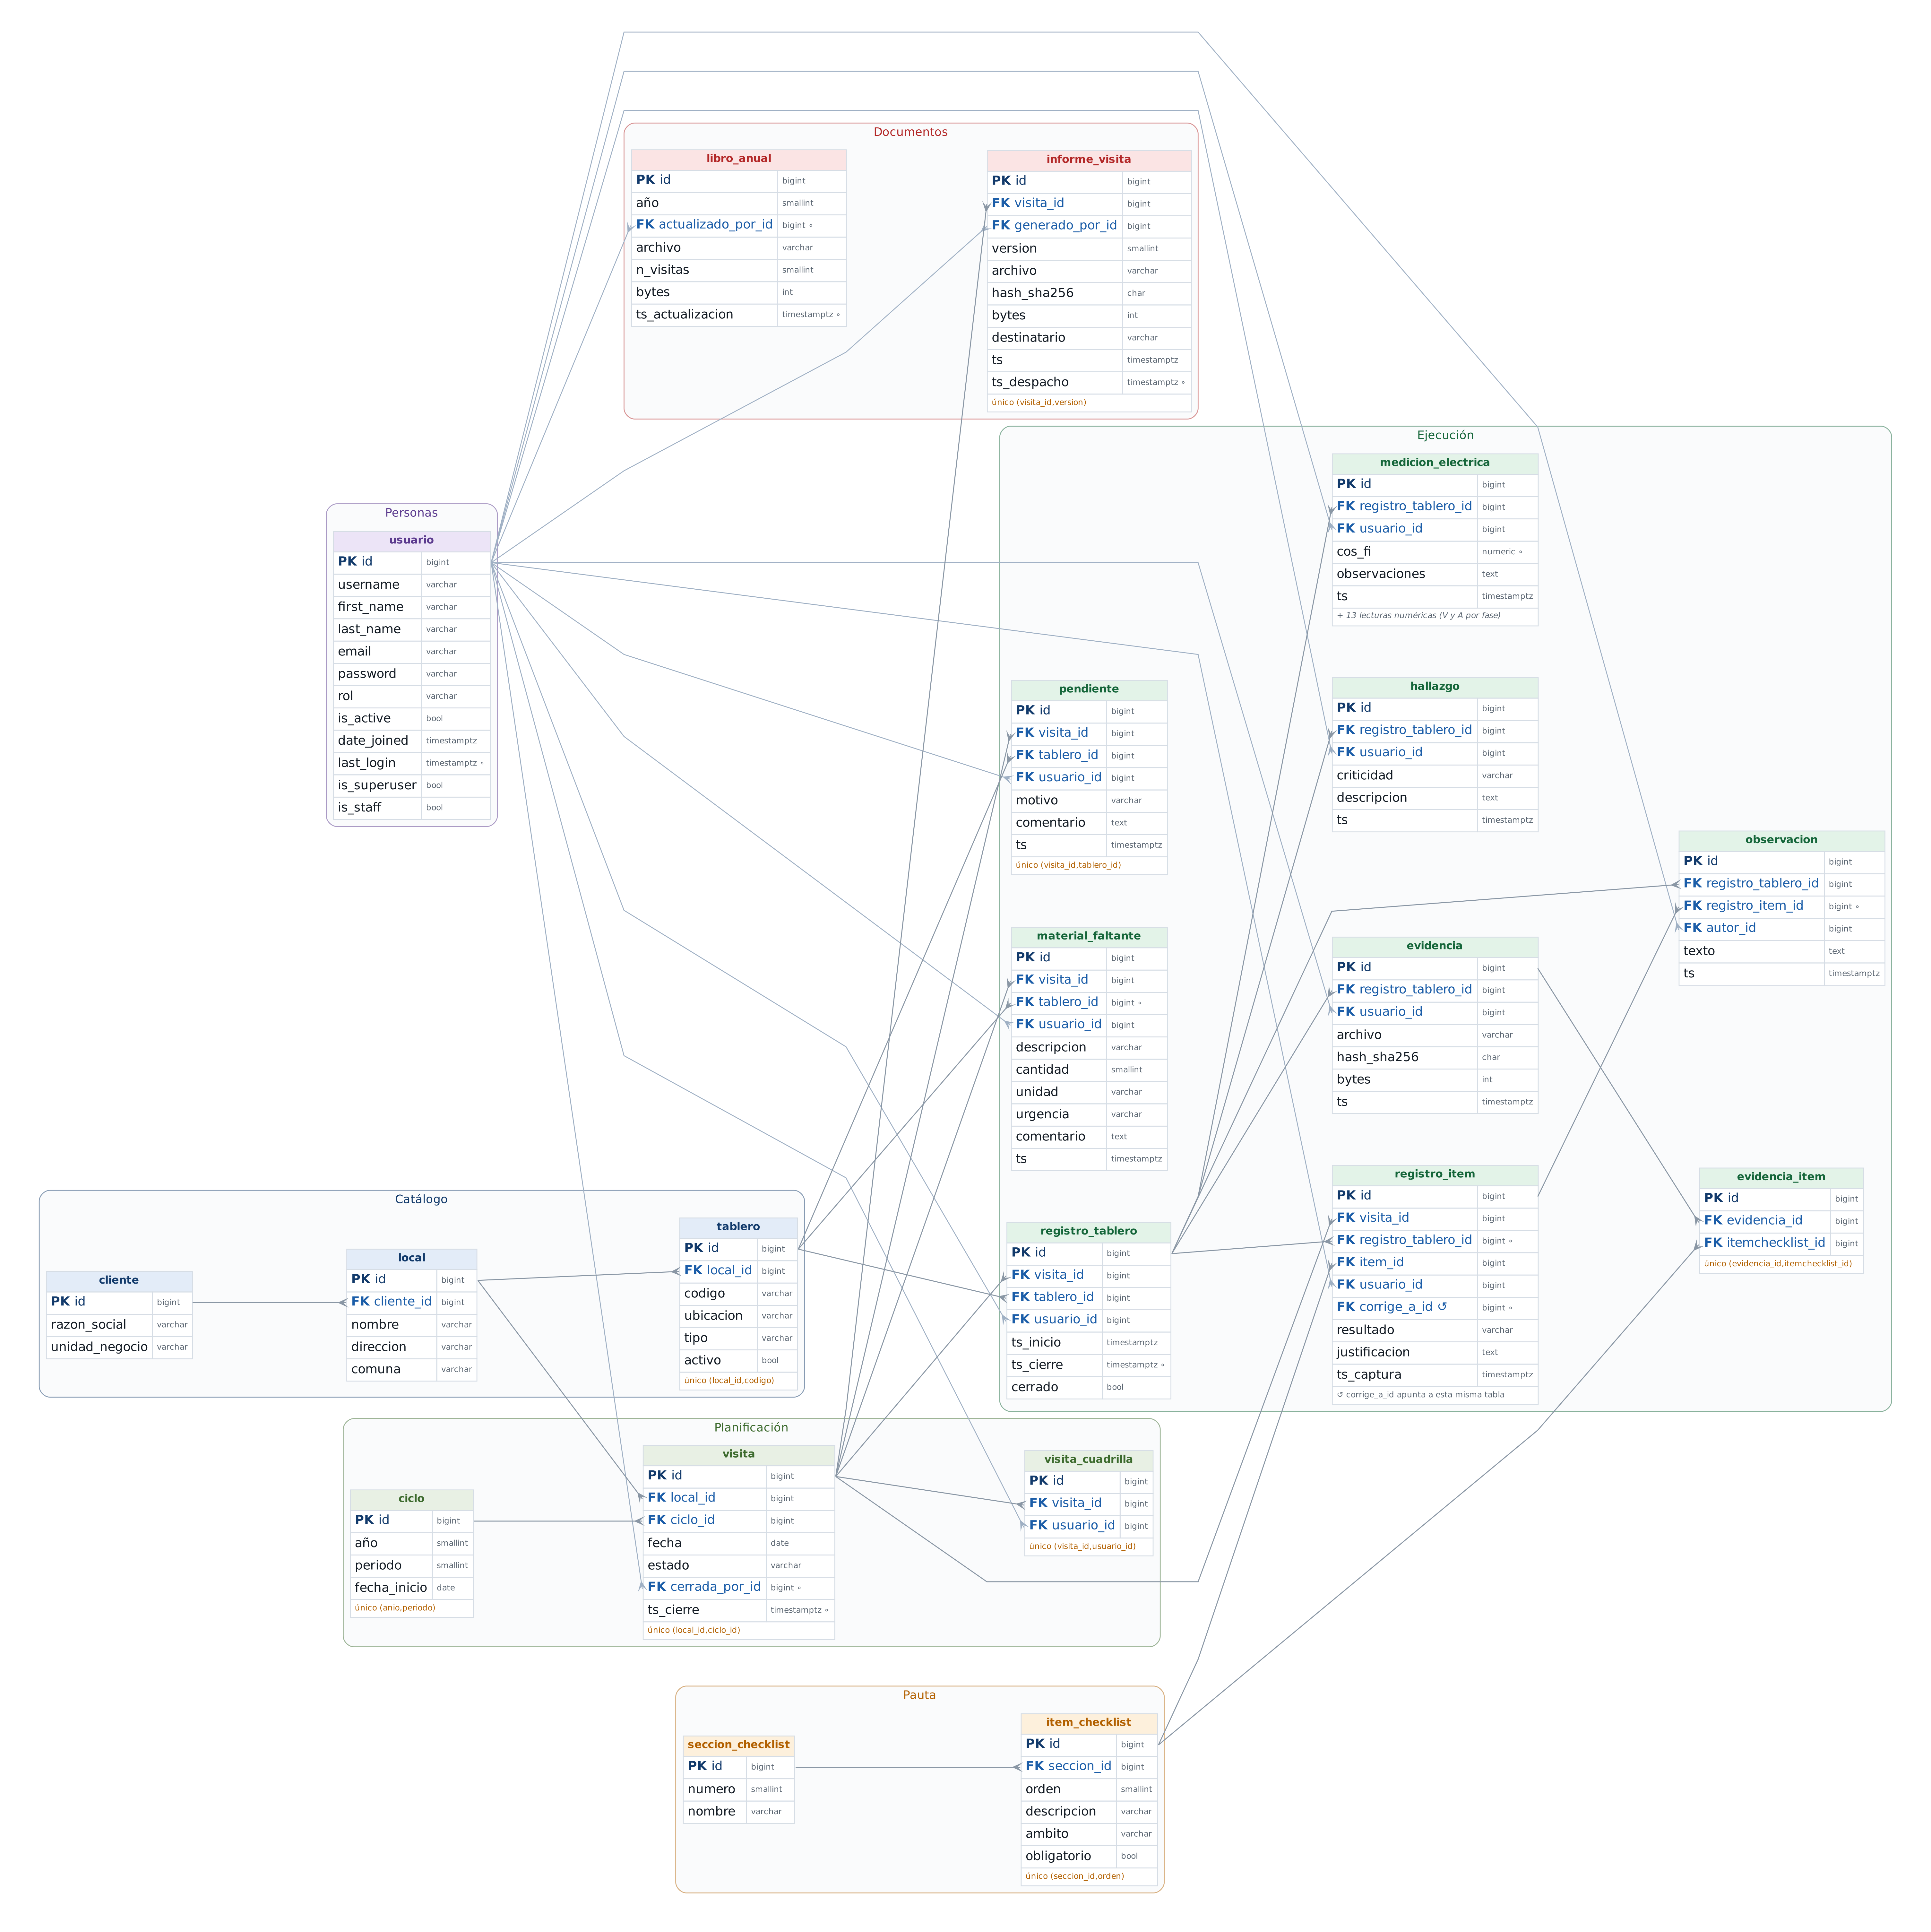
\includegraphics[height=0.7\textheight,width=\textwidth,keepaspectratio]{er-modelo-datos.png}
\caption{Modelo entidad-relación. 20 entidades de negocio, 36 relaciones,
agrupadas por área. En naranja, las restricciones de unicidad compuesta, que
son donde viven las reglas del negocio. Versión ampliable en
\texttt{docs/diagramas/}.}
\end{figure}
\newpage
\subsection{Las seis áreas}

\textbf{Personas.} Una entidad, \texttt{usuario}, referenciada por nueve
tablas: toda acción queda atribuida a una persona identificada.

\textbf{Catálogo.} \texttt{cliente} $\to$ \texttt{local} $\to$
\texttt{tablero}. La existencia de la tabla \texttt{tablero} \emph{es} la
solución del problema ya que el papel no sabe cuántos tableros tiene un local, y por
eso no puede detectar que falta uno.

\textbf{Pauta.} Los 25 puntos de control viven como datos y no escritos dentro
del código. El atributo \texttt{ámbito} separa los 10 ítems que se responden
una vez por visita de los 15 que van tablero por tablero, que es exactamente la
trazabilidad que el papel no permitía.

\textbf{Planificación.} \texttt{ciclo} y \texttt{visita}, más la relación N:M
con la cuadrilla.

\textbf{Ejecución.} Ocho entidades, todas \emph{append-only}.

\textbf{Documentos.} \texttt{informe\_visita} y \texttt{libro\_anual}.

\subsection{Normalización}

El modelo está en \textbf{tercera forma  3FN}.
\begin{enumerate}
\item \textbf{Primera forma normal.} Todos los atributos son atómicos. El caso que lo
pone a prueba es la cuadrilla: guardar «Pérez, Soto» en un campo de texto
habría violado la 1FN y haría imposible responder cuántas visitas hizo cada
técnico. Se modeló como relación N:M. El mismo criterio se aplicó a la relación
entre una fotografía y los ítems que respalda.

 \item  \textbf{Segunda forma normal.} Se cumple por construcción, porque todas las
claves primarias son simples. Donde el negocio exige unicidad compuesta
\texttt{(local, código)} en tablero, \texttt{(local, ciclo)} en visita se
declara como restricción \texttt{UNIQUE} y no como clave primaria, por las
razones de la sección 4.4.

 \item \textbf{Tercera forma normal.} No hay dependencias transitivas. La comuna está
en \texttt{local} y no copiada en \texttt{visita}. El texto del ítem está en
\texttt{ítem\_checklist} y no repetido en las 1.805 filas de
\texttt{registro\_item}. La razón social está en \texttt{cliente} y no copiada
en \texttt{local}.
\end{enumerate}

\subsubsection*{Anomalías evitadas}
\begin{itemize}
\item \textbf{De actualización.} Corregir la redacción de un punto de la pauta obligaría, en un modelo desnormalizado, a actualizar cada fila donde ese textoesté copiado, y bastaría una sin actualizar para que la base se contradiga.Aquí el texto vive en una fila y las 1.805 respuestas lo referencian.
\item \textbf{De inserción.} En un modelo donde el tablero sólo existiera como un campo dentro del registro de la mantención, no se podría registrar un tablero hasta hacerle una visita. \textbf{Esto no es un refinamiento teórico:} un modelo así no puede, por definición, detectar la ausencia de mantención, que es el problema entero del proyecto. El sistema necesita conocer los tableros que \emph{deberían} revisarse para detectar los que no se revisaron.
\item \textbf{De borrado.} Eliminar la última visita de un local podría arrastrar los datos del local. Se evita por dos mecanismos combinados: las entidades son independientes y todas las claves foráneas usan \texttt{ON DELETE RESTRICT}, de modo que la base se niega a borrar una fila referenciada. A eso se suma que las tablas de ejecución son \emph{append-only}. Un usuario que deja la empresa se marca inactivo y conserva todo lo que registró.
\end{itemize}

\newpage
\subsection{Decisiones de diseño}

\subsubsection*{Claves primarias subrogadas}

El código del tablero parece una clave natural perfecta y no se usa como tal,
por tres razones. Es un dato de terreno que puede corregirse, y el levantamiento
está incompleto en un 10 a 20\,\% de los locales. Si la clave cambiara, el
historial dejaría de apuntar a lo mismo, y el historial inmutable es la razón de
ser del sistema. Y una clave de texto se propaga a cada clave foránea, mientras
un entero es más angosto y más rápido de indexar.

La forma corta: \textbf{la clave subrogada protege la identidad de la fila, el
índice único protege la regla del negocio.}

\subsubsection*{Inmutabilidad}

Ninguna fila de las tablas de ejecución se actualiza ni se elimina tras
sellarse. Una corrección es una fila nueva encadenada a la original, con su
propio autor y fecha. Ambas quedan en la tabla.

La regla vive en la capa de datos y no en la interfaz, y la distinción importa:
esconder el botón de editar no es una regla sino una sugerencia, porque
quedarían abiertas la consola de administración, el acceso directo a la base y
cualquier funcionalidad que se escriba después sin recordar la restricción.
Puesta en el modelo, las tres puertas se cierran de una vez.

\subsubsection*{Dos denormalizaciones deliberadas}

Un modelo que declara 3FN y esconde sus excepciones se defiende peor que uno
que las nombra. Hay dos.

El \textbf{hash y el tamaño} en \texttt{evidencia} son derivables del archivo.
Se almacenan porque su valor probatorio depende de haberse calculado en el
instante de la captura: recalcularlos después daría el hash del archivo actual,
sea el original o no, lo que no probaría nada.

El campo \texttt{visita\_id} en \texttt{registro\_item} es alcanzable navegando
la relación con el registro de tablero. Se guarda directo porque los ítems de
ámbito visita no tienen registro de tablero asociado, y sin esa columna esas
230 filas quedarían huérfanas.

\subsubsection*{Las reglas del negocio como restricciones}

\begin{table}[H]
\centering
\small
\begin{tabular}{@{}p{8.5cm}p{6.5cm}@{}}
\toprule
\textbf{Regla} & \textbf{Dónde se declara} \\
\midrule
Un código de tablero es único dentro de su local & \texttt{UNIQUE (local, código)} \\
Un local se visita una vez por ciclo & \texttt{UNIQUE (local, ciclo)} \\
Una visita cerrada tiene autor y fecha de cierre & \texttt{CHECK} \\
Un ítem no conforme exige justificación & \texttt{CHECK} \\
Un pendiente con motivo «Otro» exige detalle & \texttt{CHECK} \\
Un tablero no se declara pendiente dos veces en la misma visita & \texttt{UNIQUE (visita, tablero)} \\
El factor de potencia está entre 0 y 1 & \texttt{CHECK} \\
\bottomrule
\end{tabular}
\caption{Reglas de negocio declaradas en el esquema.}
\end{table}

Un dato que viola una de estas reglas no entra a la base \textbf{venga de donde
venga}: de la aplicación, de un script o de alguien escribiendo SQL a mano.
\newpage
\subsection{Crecimiento respecto del modelo preliminar}

El modelo preliminar de la Entrega 1 tenía 12 entidades. El definitivo tiene
20.

\begin{table}[H]
\centering
\small
\begin{tabular}{@{}p{3.6cm}p{11.4cm}@{}}
\toprule
\textbf{Entidad nueva} & \textbf{Motivo} \\
\midrule
\texttt{sección\_checklist} & La ficha real agrupa sus 25 puntos en 5 secciones. \\
\texttt{registro\_tablero} & Faltaba el concepto de «lo que se sella de una vez». Sin él no hay unidad de inmutabilidad. \\
\texttt{observación} & Permite aportar sobre un registro cerrado sin alterarlo. Resuelve la objeción práctica a la inmutabilidad. \\
\texttt{evidencia\_item} & La relación foto--ítem resultó N:M. \\
\texttt{medición\_eléctrica} & Se levantó la hoja de mediciones N.º 002214. \\
\texttt{libro\_anual} & Requisito surgido durante la E2: planilla anual con hojas mensuales. \\
\texttt{informe\_visita} & El informe pasó de ser un archivo suelto a un objeto con versión y huella. \\
\texttt{material\_faltante} & El RF-11 era el único requisito que atacaba la manifestación P6 y había quedado sin implementar. \\
\bottomrule
\end{tabular}
\caption{Entidades incorporadas respecto del modelo preliminar.}
\end{table}

\subsection{Diccionario de datos}

Se omiten las columnas de infraestructura del marco de trabajo, que no forman
parte del modelo de negocio. La notación \texttt{PK} indica clave primaria,
\texttt{FK} clave foránea y $\circ$ que el atributo admite nulos.

\begin{longtable}{@{}p{2.9cm}p{3.6cm}p{1.6cm}p{6.6cm}@{}}
\toprule
\textbf{Entidad} & \textbf{Atributo} & \textbf{Clave} & \textbf{Tipo y regla} \\
\midrule
\endfirsthead
\toprule
\textbf{Entidad} & \textbf{Atributo} & \textbf{Clave} & \textbf{Tipo y regla} \\
\midrule
\endhead

\texttt{usuario} & \texttt{id} & PK & \texttt{bigint}, subrogada \\
 & \texttt{username} & & \texttt{varchar(150)}, único \\
 & \texttt{first\_name}, \texttt{last\_name} & & \texttt{varchar(150)} \\
 & \texttt{email} & & \texttt{varchar(254)} \\
 & \texttt{password} & & \texttt{varchar(128)}, cifrada con PBKDF2 \\
 & \texttt{rol} & & \texttt{TECNICO}, \texttt{ADMINISTRACION} o \texttt{GERENCIA} \\
 & \texttt{is\_active} & & \texttt{boolean}. Un usuario se desactiva, no se borra \\
\addlinespace

\texttt{cliente} & \texttt{id} & PK & \texttt{bigint} \\
 & \texttt{razón\_social} & & \texttt{varchar(120)} \\
 & \texttt{unidad\_negocio} & & \texttt{varchar(80)} \\
\addlinespace

\texttt{local} & \texttt{id} & PK & \texttt{bigint} \\
 & \texttt{cliente\_id} & FK & $\to$ \texttt{cliente}, \texttt{ON DELETE RESTRICT} \\
 & \texttt{nombre} & & \texttt{varchar(120)} \\
 & \texttt{dirección} & & \texttt{varchar(200)} \\
 & \texttt{comuna} & & \texttt{varchar(80)} \\
\addlinespace

\texttt{tablero} & \texttt{id} & PK & \texttt{bigint}, subrogada (ver 4.4) \\
 & \texttt{local\_id} & FK & $\to$ \texttt{local} \\
 & \texttt{código} & & \texttt{varchar(40)}. Único \emph{por local}, no globalmente \\
 & \texttt{ubicación} & & \texttt{varchar(150)}, ubicación física \\
 & \texttt{tipo} & & \texttt{FUERZA}, \texttt{DISTRIBUCION}, \texttt{ALUMBRADO}, \texttt{EMERGENCIA} \\
 & \texttt{activo} & & \texttt{boolean}. Un tablero retirado deja de exigirse sin perder su historial \\
\addlinespace

\texttt{sección\_} & \texttt{número} & & \texttt{smallint}, único y positivo \\
\texttt{checklist} & \texttt{nombre} & & \texttt{varchar(150)} \\
\addlinespace

\texttt{ítem\_} & \texttt{sección\_id} & FK & $\to$ \texttt{sección\_checklist} \\
\texttt{checklist} & \texttt{orden} & & \texttt{smallint}, único dentro de la sección \\
 & \texttt{descripción} & & \texttt{varchar(250)}, texto literal de la ficha N.º 002190 \\
 & \texttt{ámbito} & & \texttt{TABLERO} o \texttt{VISITA} \\
 & \texttt{obligatorio} & & \texttt{boolean} \\
\addlinespace

\texttt{ciclo} & \texttt{año} & & \texttt{smallint}, entre 2000 y 2100 \\
 & \texttt{periodo} & & \texttt{smallint}, entre 1 y 6 (bimensual) \\
 & \texttt{fecha\_inicio} & & \texttt{date} \\
\addlinespace

\texttt{visita} & \texttt{local\_id} & FK & $\to$ \texttt{local} \\
 & \texttt{ciclo\_id} & FK & $\to$ \texttt{ciclo}. Único \texttt{(local, ciclo)} \\
 & \texttt{fecha} & & \texttt{date} \\
 & \texttt{estado} & & \texttt{PLANIFICADA}, \texttt{EN\_EJECUCION}, \texttt{CERRADA} \\
 & \texttt{cerrada\_por\_id} & FK$^\circ$ & $\to$ \texttt{usuario}. Obligatorio si está cerrada \\
 & \texttt{ts\_cierre} & $\circ$ & \texttt{timestamptz}. Obligatorio si está cerrada \\
\addlinespace

\texttt{registro\_} & \texttt{visita\_id} & FK & $\to$ \texttt{visita} \\
\texttt{tablero} & \texttt{tablero\_id} & FK & $\to$ \texttt{tablero} \\
 & \texttt{usuario\_id} & FK & $\to$ \texttt{usuario}, quién lo intervino \\
 & \texttt{ts\_inicio}, \texttt{ts\_cierre} & & \texttt{timestamptz} \\
 & \texttt{cerrado} & & \texttt{boolean}. Al sellarlo el conjunto queda inmutable \\
\addlinespace

\texttt{registro\_item} & \texttt{visita\_id} & FK & $\to$ \texttt{visita} \\
 & \texttt{registro\_tablero\_id} & FK$^\circ$ & Nulo si el ítem es de ámbito visita \\
 & \texttt{ítem\_id} & FK & $\to$ \texttt{ítem\_checklist} \\
 & \texttt{usuario\_id} & FK & $\to$ \texttt{usuario} \\
 & \texttt{corrige\_a\_id} & FK$^\circ$ & Autorreferencia: la cadena de correcciones \\
 & \texttt{resultado} & & \texttt{SI}, \texttt{NO} o \texttt{NA} \\
 & \texttt{justificación} & & \texttt{text}. \textbf{Obligatoria} si el resultado no es \texttt{SI} \\
 & \texttt{ts\_captura} & & \texttt{timestamptz}, lo pone el sistema \\
\addlinespace

\texttt{evidencia} & \texttt{registro\_tablero\_id} & FK & $\to$ \texttt{registro\_tablero} \\
 & \texttt{usuario\_id} & FK & $\to$ \texttt{usuario} \\
 & \texttt{archivo} & & \texttt{varchar(100)}, ruta en el almacenamiento \\
 & \texttt{hash\_sha256} & & \texttt{char(64)}, calculado al recibir el archivo \\
 & \texttt{bytes} & & \texttt{integer}, positivo \\
 & \texttt{ts} & & \texttt{timestamptz}, lo pone el sistema \\
\addlinespace

\texttt{evidencia\_item} & \texttt{evidencia\_id} & FK & $\to$ \texttt{evidencia} \\
 & \texttt{itemchecklist\_id} & FK & $\to$ \texttt{ítem\_checklist}. Relación N:M, par único \\
\addlinespace

\texttt{observación} & \texttt{registro\_tablero\_id} & FK & $\to$ \texttt{registro\_tablero} \\
 & \texttt{registro\_item\_id} & FK$^\circ$ & Opcional, si comenta un ítem puntual \\
 & \texttt{autor\_id} & FK & $\to$ \texttt{usuario} \\
 & \texttt{texto} & & \texttt{text} \\
 & \texttt{ts} & & \texttt{timestamptz} \\
\addlinespace

\texttt{hallazgo} & \texttt{registro\_tablero\_id} & FK & $\to$ \texttt{registro\_tablero} \\
 & \texttt{criticidad} & & \texttt{BAJA}, \texttt{MEDIA}, \texttt{ALTA}, \texttt{CRITICA} \\
 & \texttt{descripción} & & \texttt{text} \\
\addlinespace

\texttt{pendiente} & \texttt{visita\_id} & FK & $\to$ \texttt{visita} \\
 & \texttt{tablero\_id} & FK & $\to$ \texttt{tablero}. Único \texttt{(visita, tablero)} \\
 & \texttt{motivo} & & Lista cerrada de seis valores \\
 & \texttt{comentario} & & \texttt{text}. Obligatorio si el motivo es \texttt{OTRO} \\
\addlinespace

\texttt{medición\_} & \texttt{registro\_tablero\_id} & FK & $\to$ \texttt{registro\_tablero}, relación 1:1 \\
\texttt{eléctrica} & 13 lecturas & & \texttt{numeric}, tensiones y corrientes por fase \\
 & \texttt{cos\_fi} & & \texttt{numeric(4,3)}, entre 0 y 1 \\
\addlinespace

\texttt{material\_} & \texttt{visita\_id} & FK & $\to$ \texttt{visita}; de ahí sale el local \\
\texttt{faltante} & \texttt{tablero\_id} & FK $\circ$ & $\to$ \texttt{tablero}. Nulo si el faltante es de consumo general del local \\
 & \texttt{descripción} & & \texttt{varchar(200)}, no vacía \\
 & \texttt{cantidad}, \texttt{unidad} & & \texttt{smallint} $\geq 1$; unidad de lista cerrada \\
 & \texttt{urgencia} & & \texttt{BLOQUEA}, \texttt{PROXIMO} o \texttt{STOCK} \\
\addlinespace

\texttt{informe\_visita} & \texttt{visita\_id} & FK & $\to$ \texttt{visita} \\
 & \texttt{versión} & & \texttt{smallint}. Único \texttt{(visita, versión)} \\
 & \texttt{archivo}, \texttt{hash\_sha256} & & El documento y su huella \\
 & \texttt{destinatario} & & \texttt{varchar(254)}, lo escribe la automatización \\
 & \texttt{ts\_despacho} & $\circ$ & Único dato que admite añadirse tras generado \\
\addlinespace

\texttt{libro\_anual} & \texttt{año} & & \texttt{smallint}, único \\
 & \texttt{archivo} & & La planilla. \textbf{Única salida que no es append-only} \\
 & \texttt{ts\_actualizacion} & & \texttt{timestamptz} \\

\bottomrule
\caption{Diccionario de datos del modelo de negocio.}
\end{longtable}

\newpage

% ============================================================
% 5. DISEÑO SQL Y RESULTADOS
% ============================================================
\section{Diseño SQL y resultados}

\subsection{Los archivos}

El esquema está en \texttt{db/schema.sql} y los datos de demostración en
\texttt{db/seed.sql}. Ambos corren sobre PostgreSQL 16 y se verificaron en una
base recién creada, sin error y con código de salida cero.

\begin{itemize}
  \item \texttt{schema.sql}: 20 tablas de negocio, 92 restricciones, con
  comentarios \texttt{COMMENT ON} en cada tabla. Incluye un apéndice separado
  con las tablas de infraestructura del marco de trabajo, de modo que una sola
  base sirva para ejecutar las consultas y para levantar la aplicación encima.
  \item \texttt{seed.sql}: un año completo de operación. Seis ciclos
  bimensuales, 4 locales, 22 tableros, 24 visitas, 105 registros de tablero
  sellados, 1.805 respuestas de la pauta y 382 evidencias.
\end{itemize}

Sobre la naturaleza de los datos: los 25 ítems de la pauta son transcripción
literal de la ficha levantada en terreno, y constituyen el único dato real.
Todo lo demás es sintético y coherente con la PYME, en cumplimiento del
compromiso declarado respecto de la Ley 21.719.

Dos situaciones se sembraron a propósito en los datos. Dos tableros acumulan
cinco ciclos consecutivos como pendientes, porque es el caso que motiva el
proyecto y sin él la consulta de seguimiento devolvería cero filas. Y el sexto
ciclo quedó en ejecución, para que las consultas de cobertura muestren un ciclo
abierto junto a cinco cerrados.

\subsection{Las reglas del negocio, escritas en el esquema}

El fragmento siguiente muestra cómo las reglas dejan de ser texto en un
documento y pasan a ser condiciones que el motor hace cumplir.

\begin{lstlisting}[language=SQL]
CREATE TABLE registro_item (
    id                  bigint      GENERATED BY DEFAULT AS IDENTITY PRIMARY KEY,
    visita_id           bigint      NOT NULL REFERENCES visita(id)         ON DELETE RESTRICT,
    registro_tablero_id bigint      REFERENCES registro_tablero(id)        ON DELETE RESTRICT,
    item_id             bigint      NOT NULL REFERENCES item_checklist(id) ON DELETE RESTRICT,
    usuario_id          bigint      NOT NULL REFERENCES usuario(id)        ON DELETE RESTRICT,
    corrige_a_id        bigint      REFERENCES registro_item(id)           ON DELETE RESTRICT,
    resultado           varchar(2)  NOT NULL,
    justificación       text        NOT NULL DEFAULT '',
    ts_captura          timestamptz NOT NULL DEFAULT now(),
    CONSTRAINT ck_regitem_resultado CHECK (resultado IN ('SI', 'NO', 'NA')),
    CONSTRAINT ck_regitem_justificacion CHECK (
        resultado = 'SI' OR length(trim(justificación)) > 0
    )
);
\end{lstlisting}

La última restricción es la simetría de la regla central del sistema, acerca de que no se declara algo hecho sin prueba, y no se declara no hecho sin decir por qué. El casillero mudo del papel no tiene equivalente posible en esta base.

La autorreferencia \texttt{corrige\_a\_id} es la cadena de correcciones. Una
respuesta corregida no se sobrescribe: la fila nueva apunta a la anterior y
ambas permanecen.

\subsection{Las consultas, ejecutadas en la aplicación}

Las seis consultas de \texttt{db/consultas/} no sólo se entregan como archivos: \textbf{La aplicación las ejecuta}. La ruta \texttt{/consultas/} lee esos mismos archivos del repositorio, los corre contra la base y muestra el resultado junto a su interpretación y al texto de la consulta. No existe una copia del SQL dentro del código, de modo que editar un archivo cambia lo que la aplicación muestra.

Esa decisión responde a la prohibición explícita de inventar resultados que la
base no pueda reproducir: la forma más corta de demostrar que no se inventó
nada es ejecutar la consulta delante de quien pregunta.

\subsection{Resultado 1: cobertura por local y ciclo}

\begin{table}[H]
\centering
\small
\begin{tabular}{@{}cccc@{}}
\toprule
\textbf{Ciclo} & \textbf{Tableros esperados} & \textbf{Registrados} & \textbf{Cobertura} \\
\midrule
1 & 22 & 19 & 86,4\,\% \\
2 & 22 & 20 & 90,9\,\% \\
3 & 22 & 19 & 86,4\,\% \\
4 & 22 & 19 & 86,4\,\% \\
5 & 22 & 19 & 86,4\,\% \\
6 \emph{(en ejecución)} & 22 & 9 & 40,9\,\% \\
\bottomrule
\end{tabular}
\caption{Cobertura agregada por ciclo. La consulta completa devuelve 24 filas,
una por local y ciclo.}
\end{table}

\textbf{Interpretación.} Éste es el indicador central del proyecto y hoy IMELSE
no puede calcularlo, porque el papel no dice a cuántos tableros se refiere una
hoja marcada. Aquí el denominador sale del listado y el numerador de los
registros sellados, de modo que el porcentaje es verificable y no declarado.

La cobertura se estabiliza en torno al 86\,\%, consistente con el 17\,\% de
mantenciones incompletas estimado en el levantamiento. La diferencia es que
ahora el número se mide.

Una visita cerrada con cobertura bajo el 100\,\% no es un error del sistema:
significa que los tableros faltantes quedaron declarados como pendientes con su
motivo, que es la única salida que el sistema permite.

\subsection{Resultado 2: tableros sin intervención}

\begin{table}[H]
\centering
\small
\begin{tabular}{@{}lllccl@{}}
\toprule
\textbf{Local} & \textbf{Tablero} & \textbf{Ubicación} & \textbf{Interv.} & \textbf{Ciclos pend.} & \textbf{Motivo recurrente} \\
\midrule
Suc. Oriente  & TD-0205 & Sala de máquinas    & \textbf{0} & 5 & Sala sin acceso \\
Suc. Centro   & TD-0407 & Entrepiso           & \textbf{0} & 5 & Equipo en operación \\
Suc. Oriente  & TD-0204 & Pasillo de cámaras  & 4 & 1 & Tiempo insuficiente \\
Suc. Poniente & TD-0304 & Pasillo de cámaras  & 4 & 1 & Tiempo insuficiente \\
Suc. Centro   & TD-0406 & Andén de carga      & 4 & 1 & Tiempo insuficiente \\
Suc. Norte    & TD-0106 & Andén de carga      & 5 & 1 & Tiempo insuficiente \\
\bottomrule
\end{tabular}
\caption{Tableros con ciclos pendientes acumulados.}
\end{table}

\begin{lstlisting}[language=SQL]
WITH ultima_intervencion AS (
    SELECT rt.tablero_id, max(v.fecha) AS fecha_ultima, count(*) AS veces_intervenido
    FROM registro_tablero rt JOIN visita v ON v.id = rt.visita_id
    WHERE rt.cerrado GROUP BY rt.tablero_id
),
pendientes_por_tablero AS (
    SELECT p.tablero_id, count(*) AS ciclos_pendiente,
           mode() WITHIN GROUP (ORDER BY p.motivo) AS motivo_recurrente
    FROM pendiente p GROUP BY p.tablero_id
)
SELECT l.nombre AS local, t.código AS tablero, t.ubicación,
       coalesce(u.veces_intervenido, 0) AS veces_intervenido,
       u.fecha_ultima AS ultima_intervencion,
       coalesce(pp.ciclos_pendiente, 0) AS ciclos_pendiente,
       pp.motivo_recurrente,
       CASE WHEN u.fecha_ultima IS NULL THEN NULL
            ELSE round((CURRENT_DATE - u.fecha_ultima) / 30.0, 1) END
            AS meses_sin_intervencion
FROM tablero t
JOIN local l                        ON l.id = t.local_id
LEFT JOIN ultima_intervencion u     ON u.tablero_id = t.id
LEFT JOIN pendientes_por_tablero pp ON pp.tablero_id = t.id
WHERE t.activo AND coalesce(pp.ciclos_pendiente, 0) > 0
ORDER BY pp.ciclos_pendiente DESC NULLS LAST, meses_sin_intervencion DESC NULLS FIRST;
\end{lstlisting}

\textbf{Interpretación.} Ésta es la consulta que justifica el proyecto
completo. El diagnóstico afirmaba que hay tableros que pasan ciclos enteros sin
revisión y que nadie se entera hasta que fallan. Con el papel esa afirmación no
se podía comprobar.
\newpage
TD-0205 y TD-0407 tienen \textbf{cero intervenciones en todo el año}. Cinco
ciclos bimensuales consecutivos equivalen a diez meses descubiertos, y cuando
uno de esos tableros falle, la visita de emergencia la paga IMELSE.

El motivo recurrente separa dos problemas que exigen decisiones distintas:
\begin{enumerate}
    \item TD-0205 queda fuera por sala sin acceso cinco veces seguidas, lo que es un problema de coordinación que se resuelve con una llamada previa.
    \item TD-0407 queda fuera por equipo en operación, lo que es un problema contractual y exige negociar una ventana de desenergización.
\end{enumerate}
  Las otras cuatro filas son pendientes
aislados por tiempo insuficiente, que es ruido operativo normal.

Sin esta consulta, los seis casos se ven igual. Con ella, dos son urgentes y
cuatro no.

\subsection{Resultado 3: latencia del registro}

\begin{table}[H]
\centering
\small
\begin{tabular}{@{}lcccc@{}}
\toprule
& \textbf{Visitas} & \textbf{Promedio} & \textbf{Mínimo} & \textbf{Máximo} \\
\midrule
Sistema & 21 & \textbf{6,8 min} & 3 min & 11 min \\
Proceso en papel (línea base E1) & --- & 16 a 24 h & --- & --- \\
\bottomrule
\end{tabular}
\caption{Latencia entre la ejecución en terreno y la disponibilidad en oficina.}
\end{table}

\textbf{Interpretación.} El papel viaja con la cuadrilla, alguien lo transcribe
y recién entonces se arma el informe. Durante esas horas, la gerencia no tiene
forma de saber qué pasó en terreno.

La razón de fondo del cambio conviene decirla con precisión: no se optimizó el
paso de traspaso, \textbf{el paso dejó de existir}. Al cerrar la visita, la
evidencia ya está en la base. Los 6,8 minutos promedio son el tiempo entre
sellar el último tablero y apretar el botón de cerrar.

Son unos 950 minutos ahorrados por visita. Con 30 visitas mensuales, alrededor
de 475 horas al mes de información que antes estaba en tránsito.

\subsection{Resultado 4: motivos de pendiente}

\begin{table}[H]
\centering
\small
\begin{tabular}{@{}llccc@{}}
\toprule
\textbf{Local} & \textbf{Motivo} & \textbf{Veces} & \textbf{Ciclos} & \textbf{\% del local} \\
\midrule
Suc. Centro   & Equipo en operación  & 5 & 5 & 83,3\,\% \\
Suc. Centro   & Tiempo insuficiente  & 1 & 1 & 16,7\,\% \\
Suc. Oriente  & Sala sin acceso      & 5 & 5 & 83,3\,\% \\
Suc. Oriente  & Tiempo insuficiente  & 1 & 1 & 16,7\,\% \\
Suc. Norte    & Tiempo insuficiente  & 1 & 1 & 100\,\% \\
Suc. Poniente & Tiempo insuficiente  & 1 & 1 & 100\,\% \\
\bottomrule
\end{tabular}
\caption{Motivos declarados de no intervención, por local.}
\end{table}

\textbf{Interpretación.} Con el papel, un tablero no intervenido quedaba como
un casillero en blanco que nadie podía interpretar. El sistema obliga a
declarar el motivo desde una lista cerrada, lo que convierte el silencio en
información agregable.

Cada motivo apunta a una decisión distinta. «Sala sin acceso» concentrado en un
local es coordinación. «Equipo en operación» concentrado es contractual.
«Tiempo insuficiente» repartido es planificación de rutas. «Falta de material»
sería un problema de bodega y conectaría con la manifestación P6, pero no
aparece en este período.

En estos datos, el 83\,\% de los pendientes de Centro y de Oriente se explican
por una sola causa cada uno, repetida todos los ciclos. Son dos conversaciones
puntuales con el cliente, no un problema sistémico de la cuadrilla.

\subsection{Resultado 5: puntos de la pauta que más fallan}

\begin{table}[H]
\centering
\small
\begin{tabular}{@{}clccc@{}}
\toprule
\textbf{Código} & \textbf{Ítem} & \textbf{No conformes} & \textbf{\%} & \textbf{Locales} \\
\midrule
2.2 & Limpieza de sala eléctrica              & 3  & 13,0\,\% & 3 \\
4.6 & Reapriete de borneras                   & 11 & 10,5\,\% & 4 \\
3.3 & Estado de interruptores tripolares      & 11 & 10,5\,\% & 4 \\
5.1 & Medición de baterías                    & 2  & 8,7\,\%  & 2 \\
5.5 & Revisión del TTA del grupo operativo    & 2  & 8,7\,\%  & 1 \\
\bottomrule
\end{tabular}
\caption{Cinco puntos de la pauta con mayor tasa de no conformidad. La consulta
completa devuelve 23 filas.}
\end{table}

\textbf{Interpretación.} El sistema registra el resultado de cada punto por
separado, lo que permite agregar algo que el papel nunca permitió.

Los dos ítems con más no conformidades aparecen en los cuatro locales. Que el problema esté repartido y no concentrado sugiere desgaste normal de componentes y no una falla de instalación. Si en cambio el mismo ítem se concentrara en un local, no sería un problema de la cuadrilla sino de la instalación de ese local, y convendría plantearlo al cliente \emph{antes} de que algo falle. Esa distinción es la que habilita la detección temprana.

\subsubsection*{Un control de calidad del propio registro}

La consulta devuelve además la columna \texttt{sin\_evidencia}: ítems
declarados como ejecutados sin fotografía vinculada.

\textbf{El resultado es cero en los 25 ítems, sobre 1.805 respuestas.}

Eso no es buena voluntad de los técnicos es que el sistema no permite sellar un tablero con ítems marcados «Sí» sin evidencia que los respalde. Esta columna verifica que la regla se sostiene sobre todos los datos y no sólo en el caso que se muestra en la demostración.

\subsection{Resultado 6: materiales por comprar}

\begin{table}[H]
\centering
\small
\begin{tabular}{@{}llccl@{}}
\toprule
\textbf{Local} & \textbf{Material} & \textbf{Cant.} & \textbf{Veces} & \textbf{Acción} \\
\midrule
Suc. Centro    & Barra de tierra de cobre 1 m   & 1  & 1 & Comprar ahora (TD-0406 detenido) \\
Suc. Norte     & Automático diferencial 2x25A   & 1  & 1 & Comprar ahora (TD-0103 detenido) \\
Suc. Oriente   & Automático diferencial 2x25A   & 1  & 1 & Comprar ahora (TD-0202 detenido) \\
Suc. Poniente  & Automático diferencial 2x25A   & 1  & 1 & Comprar ahora (TD-0301 detenido) \\
\textbf{Suc. Oriente} & \textbf{Prensaestopa PG-16} & \textbf{12} & \textbf{3} & \textbf{Subir al stock permanente} \\
Suc. Centro    & Cinta aislante autofundente    & 4  & 2 & Subir al stock permanente \\
\bottomrule
\end{tabular}
\caption{Materiales declarados como faltantes en terreno, agrupados por local.
La consulta completa devuelve 12 filas.}
\end{table}

\textbf{Interpretación.} Que el técnico registre el faltante no evita por sí
solo el re-trabajo. Lo evita que abastecimiento vea la lista agrupada
\emph{antes} de volver al local, y la columna de acción es la que convierte el
registro en una decisión.

Las cuatro primeras filas son materiales que dejaron un tablero sin poder
mantenerse: la cobertura del ciclo siguiente depende de esas compras, de modo
que no son reposiciones de rutina sino condiciones para cumplir el contrato.

La quinta fila es el hallazgo. La prensaestopa PG-16 faltó \textbf{tres veces
en Sucursal Oriente}, en los ciclos 1, 3 y 5. Eso no es un olvido puntual sino
un error de stock permanente de la camioneta, y la decisión correcta no es
comprarla una cuarta vez sino subirla al inventario base. El checklist en papel
no podía mostrarlo porque cada hoja se miraba sola: la repetición sólo aparece
al agrupar por local y contar las veces.

La relación con el resultado 2 es directa y conviene enunciarla. Aquella
consulta dice \textbf{qué tablero está detenido}; ésta dice \textbf{qué hay que
comprar para soltarlo}.


\newpage

% ============================================================
% 6. GUÍA BREVE
% ============================================================
\section{Guía breve del trabajo}

\subsection{Reproducir los resultados}

Desde un clon limpio del repositorio, con PostgreSQL 16 instalado, todos los
resultados de la sección 5 se reproducen con cuatro comandos:

\begin{lstlisting}[language=bash]
git clone https://github.com/IMicit/ICN292_T3_20262.git
cd ICN292_T3_20262
createdb sig_imelse
psql -d sig_imelse -f db/schema.sql
psql -d sig_imelse -f db/seed.sql
for f in db/consultas/*.sql; do psql -d sig_imelse -f "$f"; done
\end{lstlisting}

El procedimiento detallado, los usuarios de prueba y cómo levantar la
aplicación sobre esa misma base están en el \texttt{README.md} del repositorio.

\subsection{Organización del repositorio}

\begin{table}[H]
\centering
\small
\begin{tabular}{@{}p{3.4cm}p{11.6cm}@{}}
\toprule
\textbf{Ruta} & \textbf{Contenido} \\
\midrule
\texttt{db/} & Esquema, datos de demostración y las seis consultas. \\
\texttt{docs/} & Caso, requisitos, BPMN, modelo de datos, consultas interpretadas, automatización, instalación y declaración de uso de IA. \\
\texttt{docs/diagramas/} & Modelo entidad-relación en PNG, SVG y PDF. \\
\texttt{docs/n8n/} & Flujo de automatización exportado. \\
\texttt{app/} & Prototipo Django 5 sobre PostgreSQL 16. \\
\texttt{informe/} & Este informe, en PDF y en \LaTeX. \\
\texttt{assets/} & Diagramas BPMN y evidencia del levantamiento en terreno. \\
\bottomrule
\end{tabular}
\caption{Organización del repositorio.}
\end{table}

\subsection{Versiones}

PostgreSQL 16 como motor de base de datos. Python 3.12 o superior, Django
5.2.6, Pillow 11.3.0, reportlab 5.0.1 y openpyxl 3.1.5 para el prototipo. n8n
1.x para la automatización.

\newpage

% ============================================================
% 7. LECCIONES Y LIMITACIONES
% ============================================================
\section{Lecciones aprendidas y limitaciones}

\subsection{Un conflicto entre dos requisitos propios}

La lección más útil de esta entrega salió de un error.
El RF-03 exige que el sistema no permita marcar un ítem como ejecutado sin
registrar su evidencia asociada. El RNF-03, priorizado como \emph{Must},
establece que registrar un tablero no debe requerir más de cinco interacciones del operador. Ambos se escribieron en la Entrega 1 y ambos parecían razonables.

Son incompatibles. Al implementar RF-03 de forma estricta, es decir, con evidencia vinculada por cada ítem declarado ejecutado, el registro de un tablero pasó a requerir bastante más de cinco interacciones. La primera implementación había resuelto la tensión con un botón de marcado en bloque, que efectivamente dejaba el registro en tres acciones, pero que permitía declarar quince puntos de control como cumplidos sin haber verificado ninguno.

Se optó por \textbf{privilegiar la verificabilidad y declarar el incumplimiento del RNF-03}, por una razón de fondo: un registro rápido que no prueba nada reproduce exactamente el problema que el sistema existe para resolver. La velocidad era un medio, la evidencia era el fin.

La mitigación implementada es que una misma fotografía puede respaldar varios ítems, de modo que un tablero se cubre con tres o cuatro capturas y no con quince. El RNF-03 debería reformularse en términos de número de fotografías por tablero y no de interacciones totales.

La lección general: \textbf{dos requisitos pueden ser individualmente
razonables y conjuntamente imposibles}, y eso no se detecta especificando sino construyendo. Una especificación que no se implementa no está validada.

\subsection{Otras limitaciones declaradas}
\begin{itemize}
\item \textbf{El alcance probatorio de la evidencia.} El hash prueba que el archivo no cambió desde que el sistema lo recibió. No prueba que la fotografía se haya tomado en ese tablero. La apertura directa de la cámara y el rechazo de imágenes con más de quince minutos de antigüedad son medidas fuertes pero no infalibles. Para ir más allá harían falta metadatos firmados o geolocalización, fuera del alcance de esta entrega.
\item \textbf{El despacho por correo depende de credenciales externas.} El flujo de automatización está construido y probado, pero el envío efectivo requiere configurar un servidor de correo, que es configuración de despliegue y no de diseño.
\item \textbf{El sistema requiere un equipo permanentemente encendido.} Es propio de cualquier sistema web. Para la operación real, un servidor en la nube para una empresa de este tamaño tiene un costo del orden de 10 dólares mensuales, cifra que conviene contrastar con el seguro comprometido de 27.500 UF. La capa de operación sin conexión mitiga el riesgo: los técnicos no necesitan el servidor disponible mientras están dentro del local.
\item \textbf{Requisitos que quedaron sin implementar.} Los RF-15 y RF-16, arrastre automático de pendientes al ciclo siguiente y firma del encargado del local, estaban priorizados como \emph{Could have} desde la Entrega 1 y siguen pendientes. No queda ningún \emph{Must} ni \emph{Should} sin implementar.
\end{itemize}

El caso del RF-11 merece una línea, porque es el que más cambió durante la
entrega. Estaba priorizado como \emph{Should} y era el único requisito que
atacaba la manifestación P6, el re-trabajo en abastecimiento. Dejarlo fuera
habría significado entregar un sistema que no toca una de las seis
manifestaciones medidas del problema, lo que es una incoherencia entre el
diagnóstico y la solución antes que una falta de alcance. Se implementó, y la
consulta 6 muestra el hallazgo que lo justifica: hay un consumible que falta
tres veces en el mismo local, lo que no es un olvido sino un error de stock
permanente que el checklist en papel no podía detectar, porque cada hoja se
miraba sola.

\subsection{Qué sigue}

En orden de valor para IMELSE: conectar el servidor de correo para completar el
despacho automático, implementar el arrastre de pendientes al ciclo siguiente
—que los datos de la sección 5.4 muestran necesario, porque hay causas que se
repiten cinco ciclos seguidos—, agregar control de versiones a la pauta para
que un cambio en la ficha no afecte la lectura del historial, y publicar el
sistema en un servidor permanente con dominio propio.
\newpage
\subsection{Uso de inteligencia artificial}

El equipo utilizó asistentes de inteligencia artificial en el desarrollo del prototipo de la aplicación,la construcción del flujo de automatización y la redacción de la documentación, partiendo en todos los casos del levantamiento en terreno, la caracterización del problema, la especificación de requisitos y el modelado de procesos elaborados por el equipo en la Entrega 1. Las decisiones de diseño (qué automatizar, qué dejar fuera del alcance, qué motor de base de datos adoptar y
cómo resolver el conflicto detectado entre los requisitos RF-03 y RNF-03—
fueron tomadas y discutidas por los integrantes. Todo el código entregado fue ejecutado y verificado por el equipo.

\end{document}
